% !TEX root =  ../main_manuscript.tex 
\subsection{Statistical Methods}
Our aim was to develop a model for predicting the time of GS7. The available data for each patient were, age at the start of AS, all observed PSA measurements, and the history of biopsies. We wanted to account for the correlation between the PSA measurements of the same patient, and also their correlation with the time of GS7. An additional complication was that PSA values were missing once a patient obtained GS7. A commonly used model to handle these issues is the joint model for time-to-event and longitudinal data \citep{rizopoulos2012joint,tomer2019,coley2017prediction}.

\begin{figure}[!htb]
\centerline{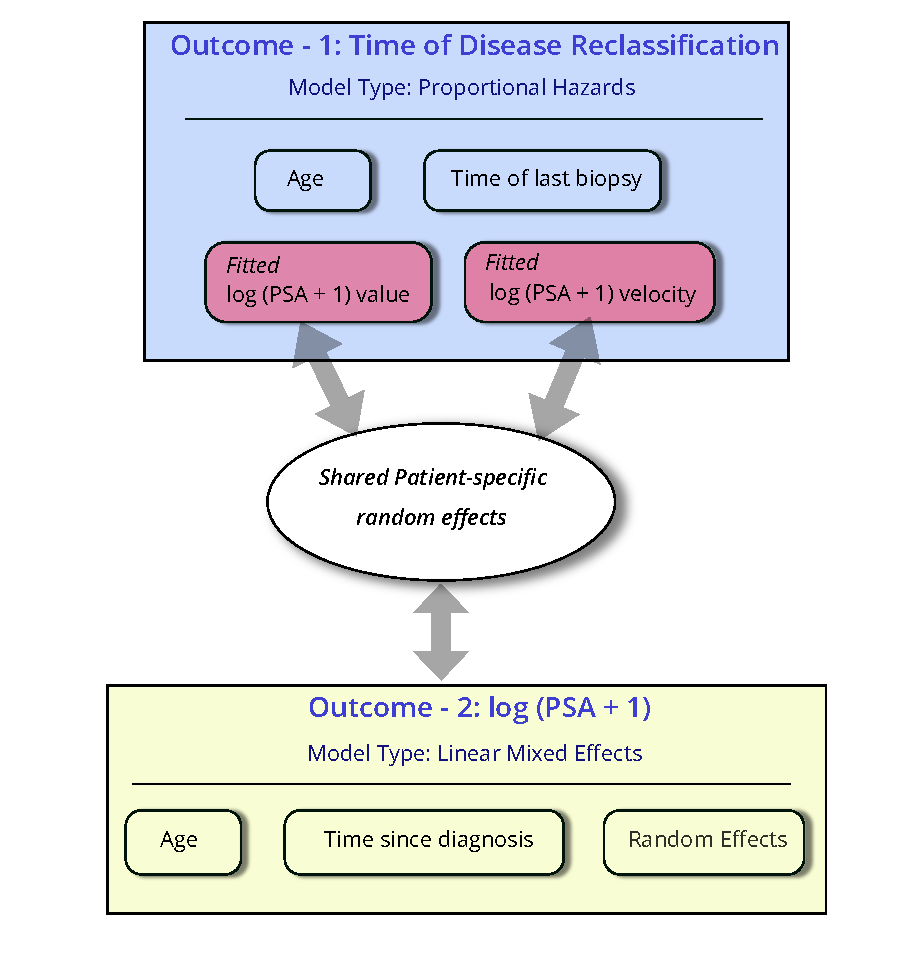
\includegraphics[width=\columnwidth]{images/jm_blockdiag.pdf}}
\caption{\textbf{Diagram of the joint model}: Patient-specific random effects (ellipse in center) are shared between sub-models for all outcomes pertaining to prostate cancer progression. The random effects model the correlation between the outcomes. In the linear mixed effects sub-model for $\log_2\{\mbox{PSA + 1}\}$ transformed PSA outcome (bottom rectangle), random effects are used as covariates. In the relative-risk sub-model (similar to Cox model) for time of Gleason~$\geq$~7 (GS7), random effects are utilized indirectly, by including fitted $\log_2\{\mbox{PSA + 1}\}$ value and velocities as covariates. Age of patient at baseline is included in both sub-models. Parameters of both sub-models are estimated jointly.}
\label{fig:jm_blockdiag}
\end{figure}

The joint model we utilized, exploited patient-specific random effects \citep{laird1982random} to act as a common source of correlation between the PSA and time of GS7 outcomes (see Figure~\ref{fig:jm_blockdiag}). Random effects also represented the underlying state of PCa, and were included in both the linear mixed effects sub-model for $\log_2\{\mbox{PSA + 1}\}$ transformed measurements, and the relative risk sub-model (similar to cox model) for time of GS7. In the PSA sub-model, random effects non-linearly modeled the evolution of PSA over time. Simultaneously, in the relative risk model they were used indirectly by including fitted $\log_2\{\mbox{PSA + 1}\}$ value and velocity as time dependent covariates. This established the correlation between PSA and time of GS7. Unlike observed $\log_2\{\mbox{PSA + 1}\}$ values, the fitted values were free of measurement errors. The $\log_2\{\mbox{PSA + 1}\}$ velocity was mathematically derived from fitted $\log_2\{\mbox{PSA + 1}\}$ values. Hence, the $\log_2\{\mbox{PSA + 1}\}$ velocity was also allowed to change non-linearly over follow-up.

The parameters of the two sub-models were estimated jointly using the R package \textbf{JMbayes} \citep{rizopoulosJMbayes}. This package utilizes the Bayesian methodology to estimate model parameters. The parameters and 95\% credible intervals are presented in Table.. of Appendix.

\subsection{Assessment of Predictions of GS7}
We validated the predictions of GS7 internally within the PRIAS dataset, as well as externally in five of the largest AS cohorts part of the GAP3 database \citep{gap3_2018}. To this end, we utilized the area under the receiver operating characteristic curve or AUC \cite{rizopoulos2017dynamic} as a measure of discrimination, and root mean squared prediction error or RMSPE \cite{rizopoulos2017dynamic} as a measure of calibration. Since AS studies are longitudinal in nature, we computed AUC and RMSPE in a time dependent manner, at a gap of every one year until xx years of follow-up (95\% quantile of observed GS7 times).

\subsection{Estimate Risk of GS7 and Consequences of Biopsies}
Consider a new patient P shown in Figure ... Using the joint model fitted to the PRIAS dataset, we obtained his cumulative risk of GS7 over the entire follow-up period. A biopsy at his current visit may be suggested if the cumulative risk of GS7 at the current visit is above a certain threshold (e.g., 10\% risk). By repeatedly applying the 10\% threshold rule over the whole follow-up, we obtained his personalized schedule of biopsies. Similar schedules can be made with another risk threshold. These schedule are not fixed but are rather updated at each follow-up visit based on newly gathered patient data. 

To assist patients in making an informed choice for a schedule, be it personalized or fixed, we provided them patient-specific consequences of following each schedule. To this end, we first calculated the probability of occurrence of GS7 between successive biopsies of each schedule. Using these probabilities we then obtained the expected delay in detection of GS7 for following that schedule. Thus, patients have a method to compare across various schedules in terms of the personalized burden (time and total biopsies), and personalized benefit (less delay in detection of GS7 is beneficial). Lastly, we implemented this approach in a web-application.

\begin{figure}[!htb]
\centerline{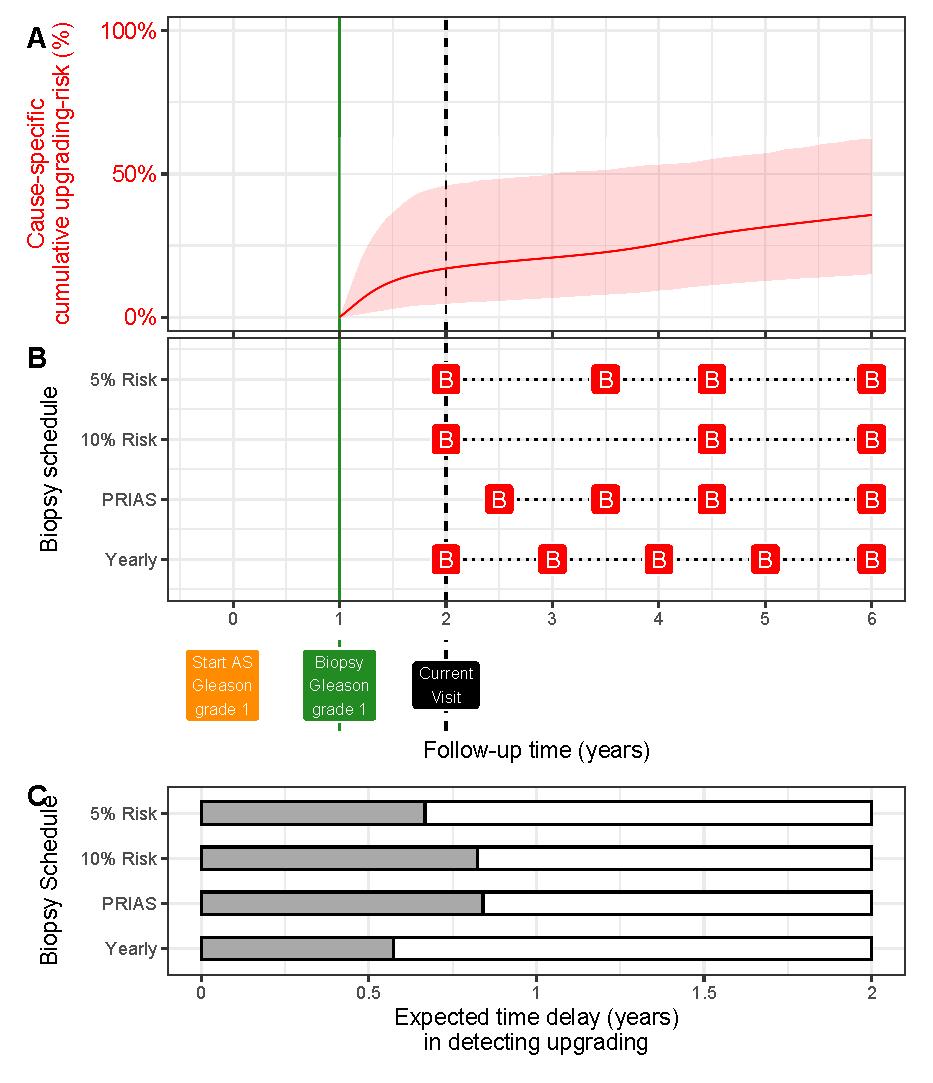
\includegraphics[width=\columnwidth]{images/demo_pat1.eps}}
\caption{}
\label{fig:demo_pat1}
\end{figure}